% !TEX TS-program = pdflatex
% !TEX encoding = UTF-8 Unicode

% This is a simple template for a LaTeX document using the "article" class.
% See "book", "report", "letter" for other types of document.

\documentclass[12pt]{article} % use larger type; default would be 10pt

\usepackage[utf8]{inputenc} % set input encoding (not needed with XeLaTeX)

%%% Examples of Article customizations
% These packages are optional, depending whether you want the features they provide.
% See the LaTeX Companion or other references for full information.

%%% PAGE DIMENSIONS
\usepackage[top=3cm,bottom=2cm,left=3cm,right=2cm]{geometry} % to change the page dimensions
\geometry{a4paper} % or letterpaper (US) or a5paper or....
% \geometry{margin=2in} % for example, change the margins to 2 inches all round
% \geometry{landscape} % set up the page for landscape
%   read geometry.pdf for detailed page layout information

\usepackage{graphicx} % support the \includegraphics command and options

\usepackage{titlesec}
\usepackage{titling}
\usepackage{lipsum}

\usepackage{indentfirst}

\titleformat{\section}
  {\bfseries}{\thesection.}{1em}{\MakeUppercase}

\titleformat{\subsection}
  {\normalfont}{\thesubsection}{1em}{\MakeUppercase}

\titleformat{\subsubsection}
  {\bfseries}{\thesubsubsection}{1em}{}

\titleformat{\paragraph}[hang]{\normalfont\normalsize\bfseries}{\theparagraph}{1em}{}
\titlespacing*{\paragraph}{0pt}{3.25ex plus 1ex minus .2ex}{0.5em}

\usepackage{tocloft}

\renewcommand{\baselinestretch}{1.50}

%\newlength{\mylen}

%\renewcommand{\cftfigpresnum}{\figurename\enspace}
%\renewcommand{\cftfigaftersnum}{:}
%\settowidth{\mylen}{\cftfigpresnum\cftfigaftersnum}
%\addtolength{\cftfignumwidth}{\mylen}

% \usepackage[parfill]{parskip} % Activate to begin paragraphs with an empty line rather than an indent

%%% PACKAGES
\usepackage[brazilian]{babel}
\usepackage{booktabs} % for much better looking tables
\usepackage{array} % for better arrays (eg matrices) in maths
\usepackage{paralist} % very flexible & customisable lists (eg. enumerate/itemize, etc.)
\usepackage{verbatim} % adds environment for commenting out blocks of text & for better verbatim
\usepackage{subfig} % make it possible to include more than one captioned figure/table in a single float
% These packages are all incorporated in the memoir class to one degree or another...
\usepackage{float}
%%% HEADERS & FOOTERS
\usepackage{fancyhdr} % This should be set AFTER setting up the page geometry
\pagestyle{fancy} % options: empty , plain , fancy
\renewcommand{\headrulewidth}{0pt} % customise the layout...
\lhead{}\chead{}\rhead{}
\lfoot{}\cfoot{\thepage}\rfoot{}

%%% SECTION TITLE APPEARANCE
%\usepackage{sectsty}
%\allsectionsfont{\sffamily\mdseries\upshape} % (See the fntguide.pdf for font help)
% (This matches ConTeXt defaults)

%%% ToC (table of contents) APPEARANCE
%\usepackage[nottoc,notlof,notlot]{tocbibind} % Put the bibliography in the ToC
%\usepackage[titles,subfigure]{tocloft} % Alter the style of the Table of Contents
%\renewcommand{\cftsecfont}{\rmfamiasly\mdseriesakdjdhaskjdasdasdasdasds\upshape}
%\renewcommand{\cftsecpagefont}{\rmfamily\mdseries\upshape} % No bold!

%%% END Article customizations

%%% The "real" document content comes below...

\title{Novas perspectivas para o diagnóstico clínico da endometriose}
\author{Clicia Santos Neves}
%\date{} % Activate to display a given date or no date (if empty),
         % otherwise the current date is printed 
\setcounter{secnumdepth}{5}
\setcounter{tocdepth}{5}         
         

\begin{document}


\begin{figure}[h!]
\centering

\includegraphics[width=4.5cm]{ibmr.png}
%\label{Rotu
\end{figure}

\begin{center}
\textbf{CENTRO UNIVERSITÁRIO HERMÍNIO DA SILVEIRA – IBMR \\
LAUREATE INTERNATIONAL UNIVERSITIES \\
CURSO DE BIOMEDICINA}
\end{center}

\vspace{2.5cm}

\begin{center}
\MakeUppercase{\theauthor}
\end{center}

\vspace{3.5cm}

\begin{center}
\MakeUppercase{\textbf{Novas perspectivas para o diagnóstico clínico da endometriose}}
\end{center}

\vspace{5.5cm}

\begin{center}
\MakeUppercase{Rio de Janeiro}\\
2015
\end{center}

\newpage


\begin{figure}[h!]
\centering

\includegraphics[width=4.5cm]{ibmr.png}
%\label{Rotu
\end{figure}

\begin{center}
\MakeUppercase{\textbf{Novas perspectivas para o diagnóstico clínico da endometriose}}
\end{center}

\vspace{4.5cm}
Trabalho de conclusão do curso apresentado ao Centro Universitário Hermínio da Silveira IBMR  –Laureate International Universities, como requisito parcial para a obtenção do grau de Bacharel em Biomedicina.

\vspace{2.5cm}

\theauthor

\vspace{2.5cm}

Orientador: Rômulo Medina Mattos

\vspace{2.0cm}
\begin{center}
\MakeUppercase{\textbf{Rio de Janeiro}}\\
2015
\end{center}

\newpage


\begin{figure}[h!]
\centering

\includegraphics[width=4.5cm]{ibmr.png}
%\label{Rotu
\end{figure}


\begin{center}
\MakeUppercase{\theauthor}
\end{center}

\vspace{2.0cm}

\begin{center}
\MakeUppercase{\textbf{Novas perspectivas para o diagnóstico clínico da endometriose}}
\end{center}

\vspace{2.0cm}

Aprovada em julho de 2015 por:

\vspace{9.0cm}

\begin{center}
\MakeUppercase{Rio de Janeiro}\\
2015
\end{center}

\newpage

\begin{center}
\MakeUppercase{\textbf{Agradecimentos}}
\end{center}

\newpage
\begin{center}
\MakeUppercase{\textbf{Resumo}}
\end{center}

A endometriose é uma doença benigna, enigmática e controversa. E
caracteriza-se pela presença de tecido semelhante ao endométrio ativo
e não neoplásico fora da cavidade uterina, assim induzindo uma reação
inflamatória crônica.

% Alguns autores?
Estima-se que cerca de 15\% das mulheres em idade reprodutiva são
afetadas pela endometriose, cujos variados sintomas diminuem a
qualidade de vida da paciente. É, portanto, considerada uma doença de
custo humano e financeiro grande.  Tanto por seus efeitos na vida da
paciente como no seu impacto profissional e com gastos médicos.
Assim, tornando-se um problema de saúde pública mundial.

% Quem acredita?
Porém, sua etiologia e etiopatogenia são ainda controversos. Mas
acredita-se que múltiplos fatores estejam envolvidos, sendo os mais
predominantes: os genéticos, ambientais, angiogênicos, endócrinos e
os processos embrionários.

Os implantes endometriais se apresentam de várias formas. Podendo ser
superficial, intermediária, profunda ou infiltrativa. Entretanto, a
sintomatologia não corresponde a gravidade da doença. 

O diagnóstico definitivo utilizado atualmente é através da
laparoscopia ou laparotomia e associados a histologia de
confirmação. Porém, esta é uma abordagem cirúrgica invasiva e de alto
custo. Sendo assim, outras técnicas de diagnóstico estão sendo
empregadas para detectar os focos das lesões, como: a Ultrassonografia
e a Ressonância Nuclear Magnética.

Apesar disto, a endometriose ainda não tem cura e seu tratamento é
apenas paliativo, uma vez que é uma doença com reincidia comprovada.

Sendo assim, o objetivo deste trabalho é o de realizar uma descrição
da literatura com o intuito de um melhor entendimento da doença, seu
diagnóstico convencional e a busca para abordagens de diagnósticos
precoce e minimamente invasivos.

\newpage\MakeUppercase{\textbf{Abstract}}



\newpage

\listoffigures



\newpage

\tableofcontents


\newpage







%\maketitle

\newpage


\section{Introdução}

A endometriose é uma doença benigna que acomete mulheres em idade
reprodutiva e é causada pela presença do tecido do endométrio fora do
revestimento do útero e pode ser encontrada em qualquer local da
cavidade abdominal. Porém, tem maior incidência na pelve, nas
estruturas próximas ao útero e raramente acomete outras regiões mais
distantes como pulmão, tórax e pericárdio (King, 2007). A endometriose
pode, também, apresentar características semelhantes a tumores, como a
invasão e a metástase, entretanto esse tipo de ocorrência é
rara. (Robins e Cotran, 2010).

% Quem acredita?
Cerca de 10\% a 15\% das mulheres em idade reprodutiva são afetadas
por esta doença. Seu diagnóstico é predominante em mulheres com dores
pélvicas ou inférteis (Matta e Muller, 2005).  Inclusive, a
endometriose lidera as causas de infertilidade entre mulheres com
idade acima de 25 anos (Cox e Cols, 2002) e é possível que até 40\%
das mulheres inférteis tenham algum grau de endometriose.

Os fatores que determinam o fenótipo da doença são diversos, como: a
quantidade do fluxo menstrual, fatores genéticos e ambientais (Viganò
e Cols, 2012). E, apesar de ser uma das doenças mais investigadas
atualmente, a endometriose ainda é de etiopatogenia desconhecida e seu
diagnóstico bastante controverso. Também, por apresentar sintomas
clínicos como dor pélvica crônica, dismenorreia, dispareunia e
subfertilidade, torna seu diagnóstico mais difícil porque, em geral,
mulheres com uma ou mais dessas condições só procuram ajuda médica
quando já se tem a doença estabelecida (Verkauf, 1897 ). 

Atualmente, não existe cura para a endometriose e nem um tratamento
padrão. Portanto, seu tratamento é individualizado para cada paciente
e o diagnóstico precoce é muito importante para evitar o agravamento
da doença e garantir uma qualidade de vida melhor.  Todavia, uma
pesquisa realizada por (Kelechi e Cols, 2009) verificou que há uma
demora de cerca de sete anos entre o aparecimento dos primeiros
sintomas até um diagnóstico preciso.

Para um diagnóstico definitivo é necessário uma visualização direta
das lesões por laparoscopia ou laparotomia combinado com a histologia
de confirmação. Entretanto, muitas mulheres deixam de fazer esse exame
por considerá-la uma abordagem invasiva ou desnecessária (Kennedy e
Cols 2005).  Sendo assim, afim de ter maior aceitação ao procedimento
diagnóstico, outras técnicas tem sido utilizadas para a visualização
das lesões, como a Utrassom Transvaginal e a Ressonância Magnética.

Como ainda não há consenso médico sobre as causas que levam o tecido
endometrial a se desenvolver em outros locais ao de sua origem, sua
cura é desconhecida. Entretanto, diversos estudos recentes sobre a
doença, focando nas características das mulheres com a doença ajudaram
a medicina a abrir novas frentes de conhecimento e permitiu a
classificação de sub-tipos de endometriose. E, assim, o presente
trabalho pretende expor as formas de diagnóstico mais utilizadas
atualmente e compará-las com os recentes diagnósticos para a
endometriose.

\section{Objetivo geral}

Apesar de a endometriose ser vastamente investigada, ainda sabe-se
muito pouco dela. Sem cura e com diagnóstico bastante controverso,
agrava-se pela sua variação de incidência que impossibilita ainda um
método de prevenção. Também, o desconhecimento pelas mulheres desta
doença contribui para o diagnóstico tardio e consequente perda de
qualidade de vida.

Visando avaliar seu difícil diagnóstico, este estudo tem o objetivo de
expor um melhor entendimento desta patologia onde discutiremos as
formas de diagnóstico clínico que são utilizadas atualmente e as novas
pesquisas para uma visão mais ampla sobre a endometriose na busca por
um diagnóstico precoce e minimamente invasivo.

\subsection{Objetivos específicos}

Os objetivos específicos são os seguintes:

\begin{itemize}
\item Descrever a fisiopatologia da endometriose.
\item Demonstrar atuais formas de diagnósticos e tratamento.
\item Discutir novas perspectivas para um diagnóstico precoce e menos
invasivos.
\end{itemize}

\section{Revisão bibliográfica}

\subsection{Aparelho Reprodutor Feminino}

O aparelho reprodutor feminino é o conjunto de órgãos responsáveis
pela reprodução, produção dos gametas, hormônios, preparação do
endométrio para a fecundação, alojamento do embrião caso o óvulo seja
fertilizado e à menstruação em caso contrário. Ele é de suma
importância já que é responsável pela perpetuação da espécie através
da reprodução sexuada. Os órgãos mais importantes que compõe o
aparelho reprodutor feminino são: os ovários,s a tuba uterina, útero e
a vagina (Guyton e Hall., 2006). Vide figura~\ref{aparelho feminino}
na página~\pageref{aparelho feminino}.


\begin{figure}[h!]
\centering
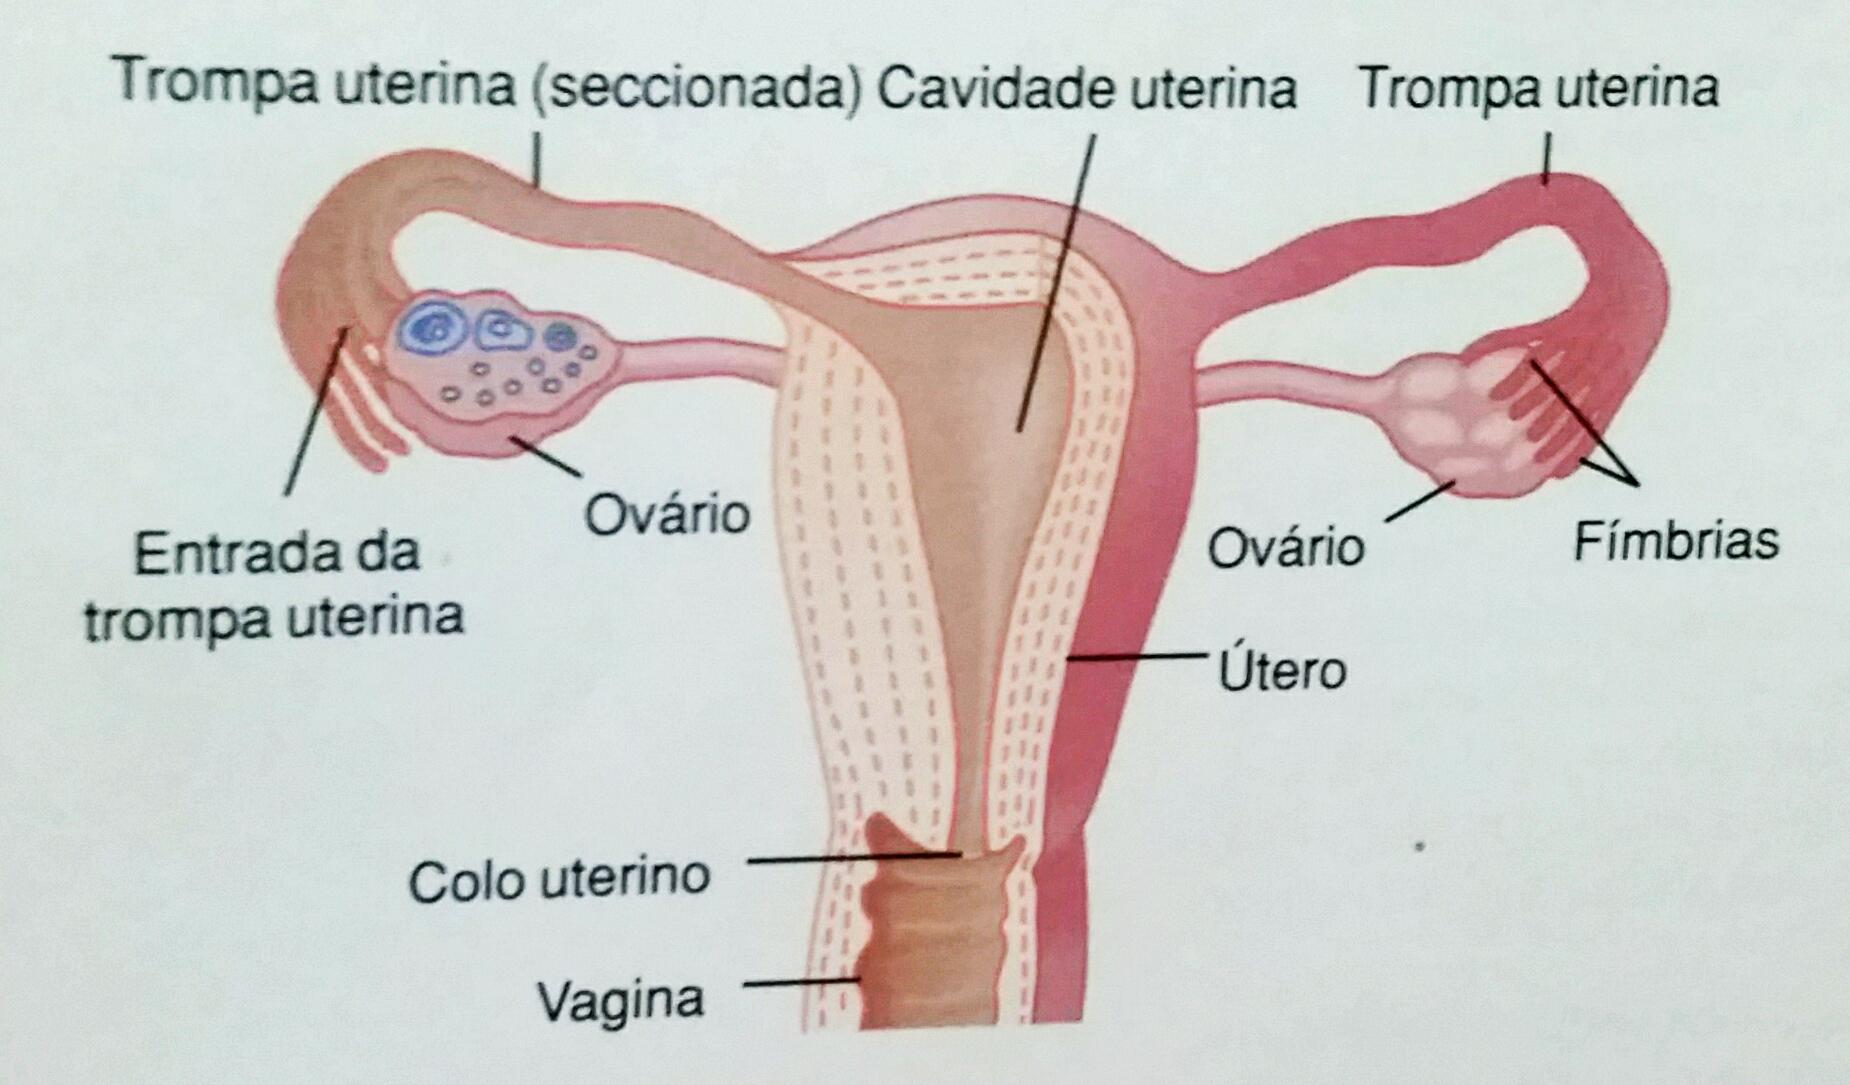
\includegraphics[width=10cm]{utero.jpg}
\caption[Anatomia do sistema reprodutor feminino]{Anatomia do sistema reprodutor feminino (Disponível em Guyton e Hall,2006 pag. 1012)}
\label{aparelho feminino}
\end{figure}

\subsection{Útero}

Um equívoco comum é o de acreditar que o útero tem como única função
abrigar o feto no período gestacional. Porém, ele também tem um papel
fundamental no ciclo ovulatório e, por isso, é também muito importante
no equilíbrio da vida da mulher.

O útero é um órgão muscular e glandular. Possui uma cavidade interna e
mede cerca de 8cm de comprimento, 5cm de largura e 3cm de
espessura. Seu formato é semelhante a uma pêra invertida e está
subdivido em três partes: fundo (região superior), corpo e colo (ou cérvix).

A parede uterina é formada por três camadas: a mais externa
constituída por mesotélio e tecido conjuntivo, o miométrio que é
constituído de músculo liso e o endométrio ou mucosa uterina
(Junqueira e Carneiro, 2008). O endométrio é um tecido vascularizado que
reveste a parede interna do útero e tem como função acolher e nutrir o
embrião na gravidez. Portanto, durante o período pré-puberal, o
tecido endometrial permanece inativo. Ele é composto por glândulas e
estroma e sofre alterações fisiológicas e morfológicas em resposta aos
hormônios ovarianos estrogênio e progesterona durante o ciclo
menstrual (Filho, 2011).  Desta forma, o útero passa por esse processo
cíclico normalmente a cada trinta dias em mulheres com idade
reprodutiva.

Há diversas teorias que tentam explicar como o endométrio vai parar
fora do útero. Uma delas é que durante a menstruação células do
endométrio invadem as trompas e com isso vão parar em vários lugares
do abdome (Robbins e Cotran, 2010).

\subsection{Ciclo menstrual}

\begin{figure}[h!]
\centering
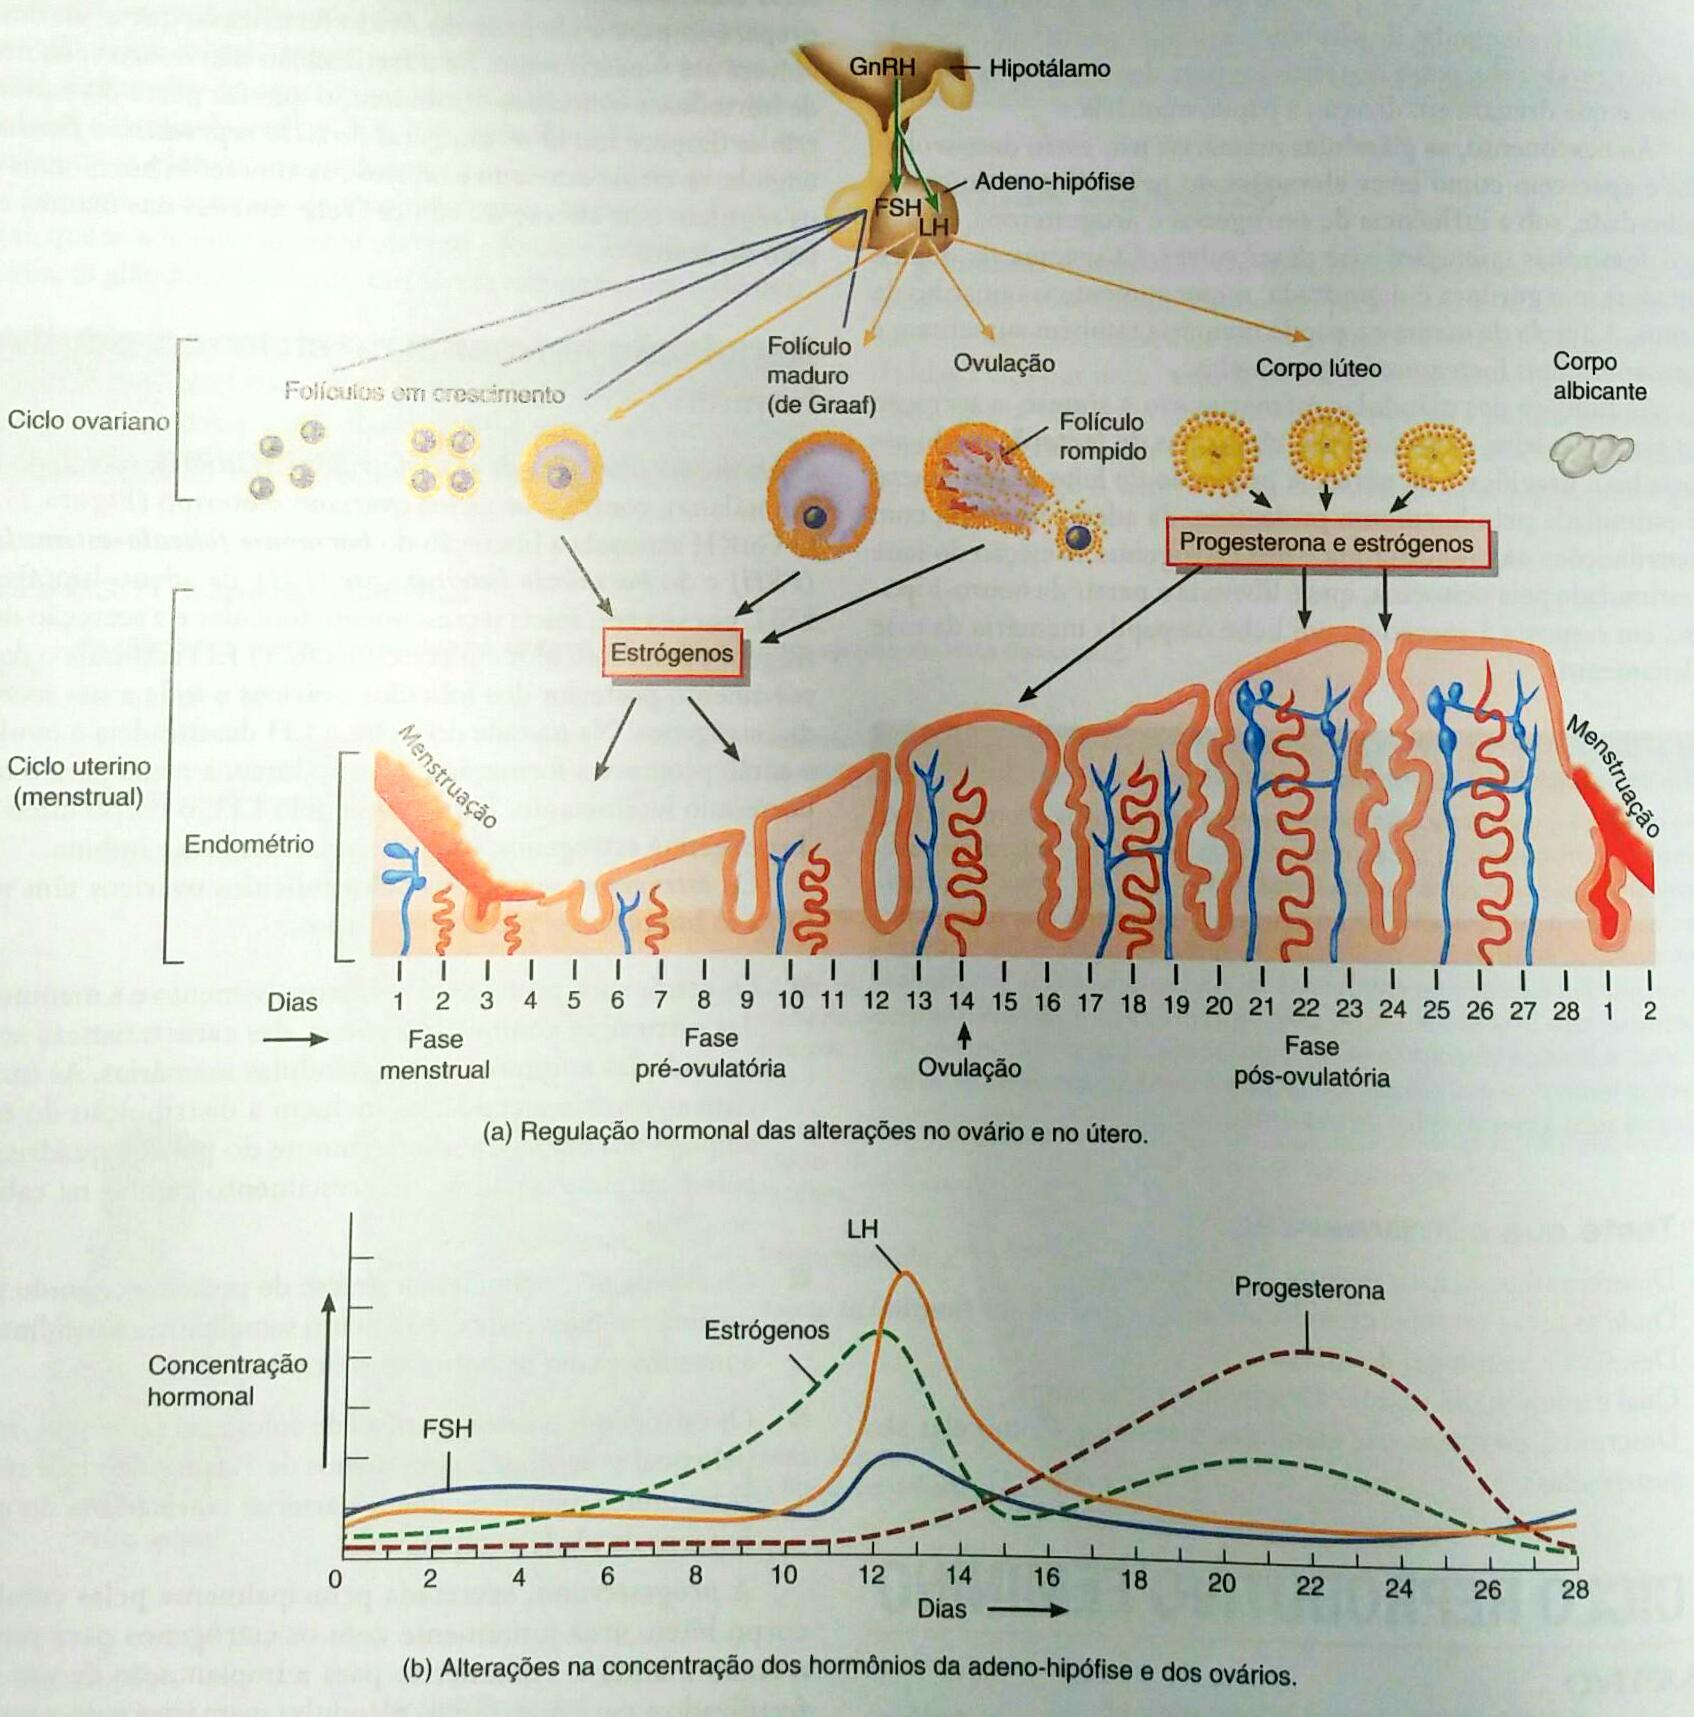
\includegraphics[width=10cm]{ciclo.jpg}
\caption[Alterações morfológicas e hormonais durante o ciclo menstrual]{ Alterações morfológicas e hormonais durante o ciclo menstrual (disponível em) } 
\label{ciclo menstrual}
\end{figure} 

Toda mulher, em seu estado fisiológico normal, em idade reprodutiva no
período entre a menarca e a menopausa, sofre alterações cíclicas em
seu sistema reprodutivo conhecido como ciclo menstrual. O ciclo
menstrual causa alterações em diversas partes do corpo feminino
incluindo mamas, útero, pele e ovários. Ele envolve um conjunto de
reações químicas endócrinas que afetam aspectos biológicos e
sociológicos como: a reprodução, sexualidade e fertilidade da
mulher. Todo o ciclo dura, em média, 28 dias e se caracteriza pela
secreção dos hormônios femininos que vão agir para a liberação do
óvulo e preparação do endométrio uterino para a implantação do óvulo,
caso seja fertilizado.

O sistema hormonal feminino, figura~\ref{ciclo menstrual} página
\pageref{ciclo menstrual}, é seguido por três hierarquias de hormônios
a serem liberados: O hormônio liberador de gonadotrofinas (GnRH),
secretado pelo hipotálamo, o hormônio folículo estimulante (FSH) e o
hormônio luteinizante (LH) que são liberados pela hipófise anterior
em resposta à liberação do GnRH e por fim os hormônios ovarianos
estrogênio e progesterona, ambos secretados pelos ovários em resposta
à liberação do FSH e do LH (Guyton e Hall, 2006).


O endométrio sofre modificações tanto histológicas quanto morfológicas
em resposta à liberação do estrogênio e da progesterona, liberados
pelos ovários durante o ciclo menstrual (Geraldo Brasileiro Filho,
2011). Essas mudanças, que tem início a cada ciclo, tem a finalidade
de preparar a parede uterina para a nidação do blastocisto caso haja a
fecundação. A primeira alteração, conhecida como fase proliferativa,
ocorre simultaneamente à fase folicular do cilo ovariano (Mattson e
Matfin, 2010).

No início de cada ciclo, o endométrio se descama preservando as
células de sua camada mais profunda. Sob a influência do estrogênio,
liberado pelos ovários, estas células endometriais da camada mais
basal se proliferam rapidamente tanto as glândulas quanto o estroma e
em poucos dias a superfície do endométrio é reepitelizada, cessando a
descamação e o sangramento (Curi e Procopio, 2009).

Por outro lado, a fase secretora acontece após a ovulação. Nos ovários
o corpo lúteo passa a produzir estrogênio e, principalmente,
progesterona. A progesterona vai atuar no endométrio estimulando a
secreção das glândulas (Mattson e Matfin, 2010) e fazendo com que o
endométrio fique ainda mais vascularizado. À medida em que a
progesterona vai predominando em relação ao estrogênio, a capacidade
proliferativa do endométrio diminui sua velocidade e a atividade
mitótica é interrompida (Karp e Jason, 2015).

Aproximadamente uma semana após a ovulação, o endométrio encontra-se
bastante vascularizado e repleto de glicogênio. As glândulas
endometriais, em sua atividade secretora máxima, % o que está pronto??
pronto para receber o óvulo fecundado. Com a não ocorrência da
fecundação, o corpo lúteo regride, e o endométrio sofre a descamação
dando início a um novo ciclo.  (Curi e Procopio, 2009).

\section{Endometriose}

A endometriose é uma doença ginecológica comum, de caráter benigno,
que se caracteriza pela presença de tecido endometrial funcional com
atividade celular evidente em: lesões, nódulos, quistos ou
endometrioma (Audebert et al., 1992) e fora da cavidade uterina, como:
ovários, ligamentos uterinos, septo vaginal, fundo de saco, peritônio
pélvico, intestino grosso e delgado (Robins e Cotran, 2010). E, embora
esses sejam os locais mais comuns, a endometriose pode, raramente,
acometer órgãos e tecidos fora da pélvis, como: bexiga, trato urinário
e até mesmo locais mais distantes como pulmão, mamas e ossos (Filho,
2012).  ( colocar uma imagem de uma lesao endometriótica)

A endometriose é uma condição crônica estrogênio-dependente que,
geralmente, acomete mulheres em idade reprodutiva (Kumar e Cols ,
2012). Apesar de ser uma doença comum e frequentemente estudada, sua
causa ainda permanece desconhecida, havendo um numero cada vez maior
de casos diagnosticados. Estima-se que a endometriose afeta de 10\% a
15\% das mulheres na pré-menopausa e de 15\% a 70\% em mulheres com
infertilidade pré-diagnosticada. Algumas condições clínicas, genéticas
e imunes podem ser ditas como fatores de risco para o aparecimento das
lesões endometriais. Alguns exemplos de condições são: o aumento da
dor e do fluxo menstrual, menarca precoce e até mesmo algum parente de
primeiro grau com a mesma condição patológica (Porth e Matfin, 2010).

As lesões endometriais ectópicas possuem tecido ativo. E respondem de
forma semelhante ao endométrio eutópico. Durante o ciclo menstrual,
podem causar hemorragias, inflamação e cicatrizes por responderem aos
estímulos dos hormônios ovarianos, o estrogênio e
progesterona. (Dongxu e Cols, 2014).

Embora as lesões endometrióticas normalmente apareçam com aspectos
benignos na histopatologia, de acordo com alguns autores, a
endometriose tem sido comparado a um tumor maligno já que as lesões
tem a capacidade de crescer, se infiltrar e aderir aos tecidos
adjacentes (Kitawaki e Cols, 2002;. Noble e Cols, 1996). Porém, ela
raramente apresenta as características de metástase e invasão
(Robins e Cotran 2010).

Entretanto, a endometriose, sendo uma doença bastante complexa, pode,
quando combinados, grupos de fatores distintos podem ter um papel
importante na fisiopatologia da doença tais como polimorfismo
genético, interferência hormonal através de receptores de estrogênios
e progesterona, fatores do sistema imunológicos e endócrinos (Troncon
e Cols, 2014).

\subsection{Classificação das lesões endometrióticas}

\subsubsection{Coloração}

Cada lesão endometrial pode caracterizar-se, macroscopicamente, de forma
diferente, variando: em sua coloração, forma e localização,
podendo ser típica, quando apresenta cor escura ou atípica
caracterizada pela cor amarelada ou avermelhada, indicando maior
atividade da doença.

Os aspectos das lesões sofrem uma variação de cor que vai da coloração
inicial amarelada para a "café com leite", até alcançar uma coloração
escura. Essa variação ocorre devido ao acúmulo de hemossiderina no
foco da lesão. Redwine, 1987 relatou que essas alterações entre a
mudança de claro até chegar ao escuro, ou cicatricial, levam em média
de 7 a 10 anos.

No ovário, o tecido endometrial pode formar cistos, conhecidos como
cistos de chocolate, pois, eles estão repletos de sangue velho que se
assemelha a calda de chocolate (Figura~\ref{implantes do endometrio},
página~\pageref{implantes do endometrio}). Em outras partes da pelve,
o tecido pode assumir a forma de pequenas lesões hemorrágicas que
podem ser: negras, azuladas, vermelhas, claras ou opacas (Porth e
Matfin ,2010).

As lesões vermelhas são altamente vascularizadas, causando sangramento
para dentro da cavidade peritoneal, aderências e inflamação. Já as
lesões mais escuras, ou brancas, representam uma lesão cicatricial
da endometriose. Do ponto de vista histológico, essas lesões são pouco
vascularizadas e estão correlacionadas com uma maior quantidade de
fibrose (Brosens, 1997).

\begin{figure}[h!] 
\centering
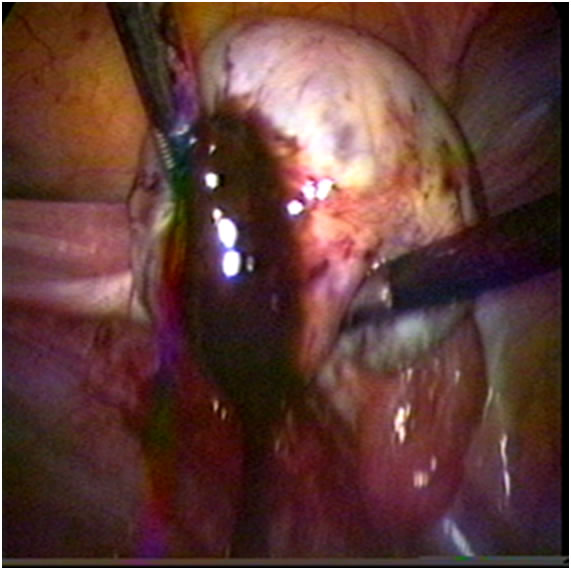
\includegraphics[width=10cm]{endometriomaroto.jpg}
\caption[Endometriose: implantes do endométrio no ovário] {implantes do endométrio no ovário (disponível em)}
\label{implantes do endometrio}
\end{figure} 


\subsubsection{Diferenciação histológica}

Porto e Cols, 2015 caracterizaram o tecido endometrial da seguinte
forma (Figura~\ref{histologico}, página~\pageref{histologico}):
Estromal, tecido com presença de estroma com aspectos morfológicos
similares ao endométrio tópico; Glandular bem diferenciada,
caracterizada por conter células epiteliais com morfologia semelhante
ao endométrio tópico; Glandular indiferenciada, tecido com epitélio
glandular plano ou cubos baixos sem correspondência com o endométrio
ectópico; Mista, tecido no qual possui a presença de glândulas de
padrão diferenciado e indiferenciado. A partir desse estudo
constataram que o tipo histológico glandular bem diferenciado
predominam nas lesões superficiais, já os tipos glandulares
indiferenciados e mistos tem uma maior prevalência nas lesões
endometrióticas profundas que acomete o peritônio e o intestino.

\begin{figure}[h!]
\centering
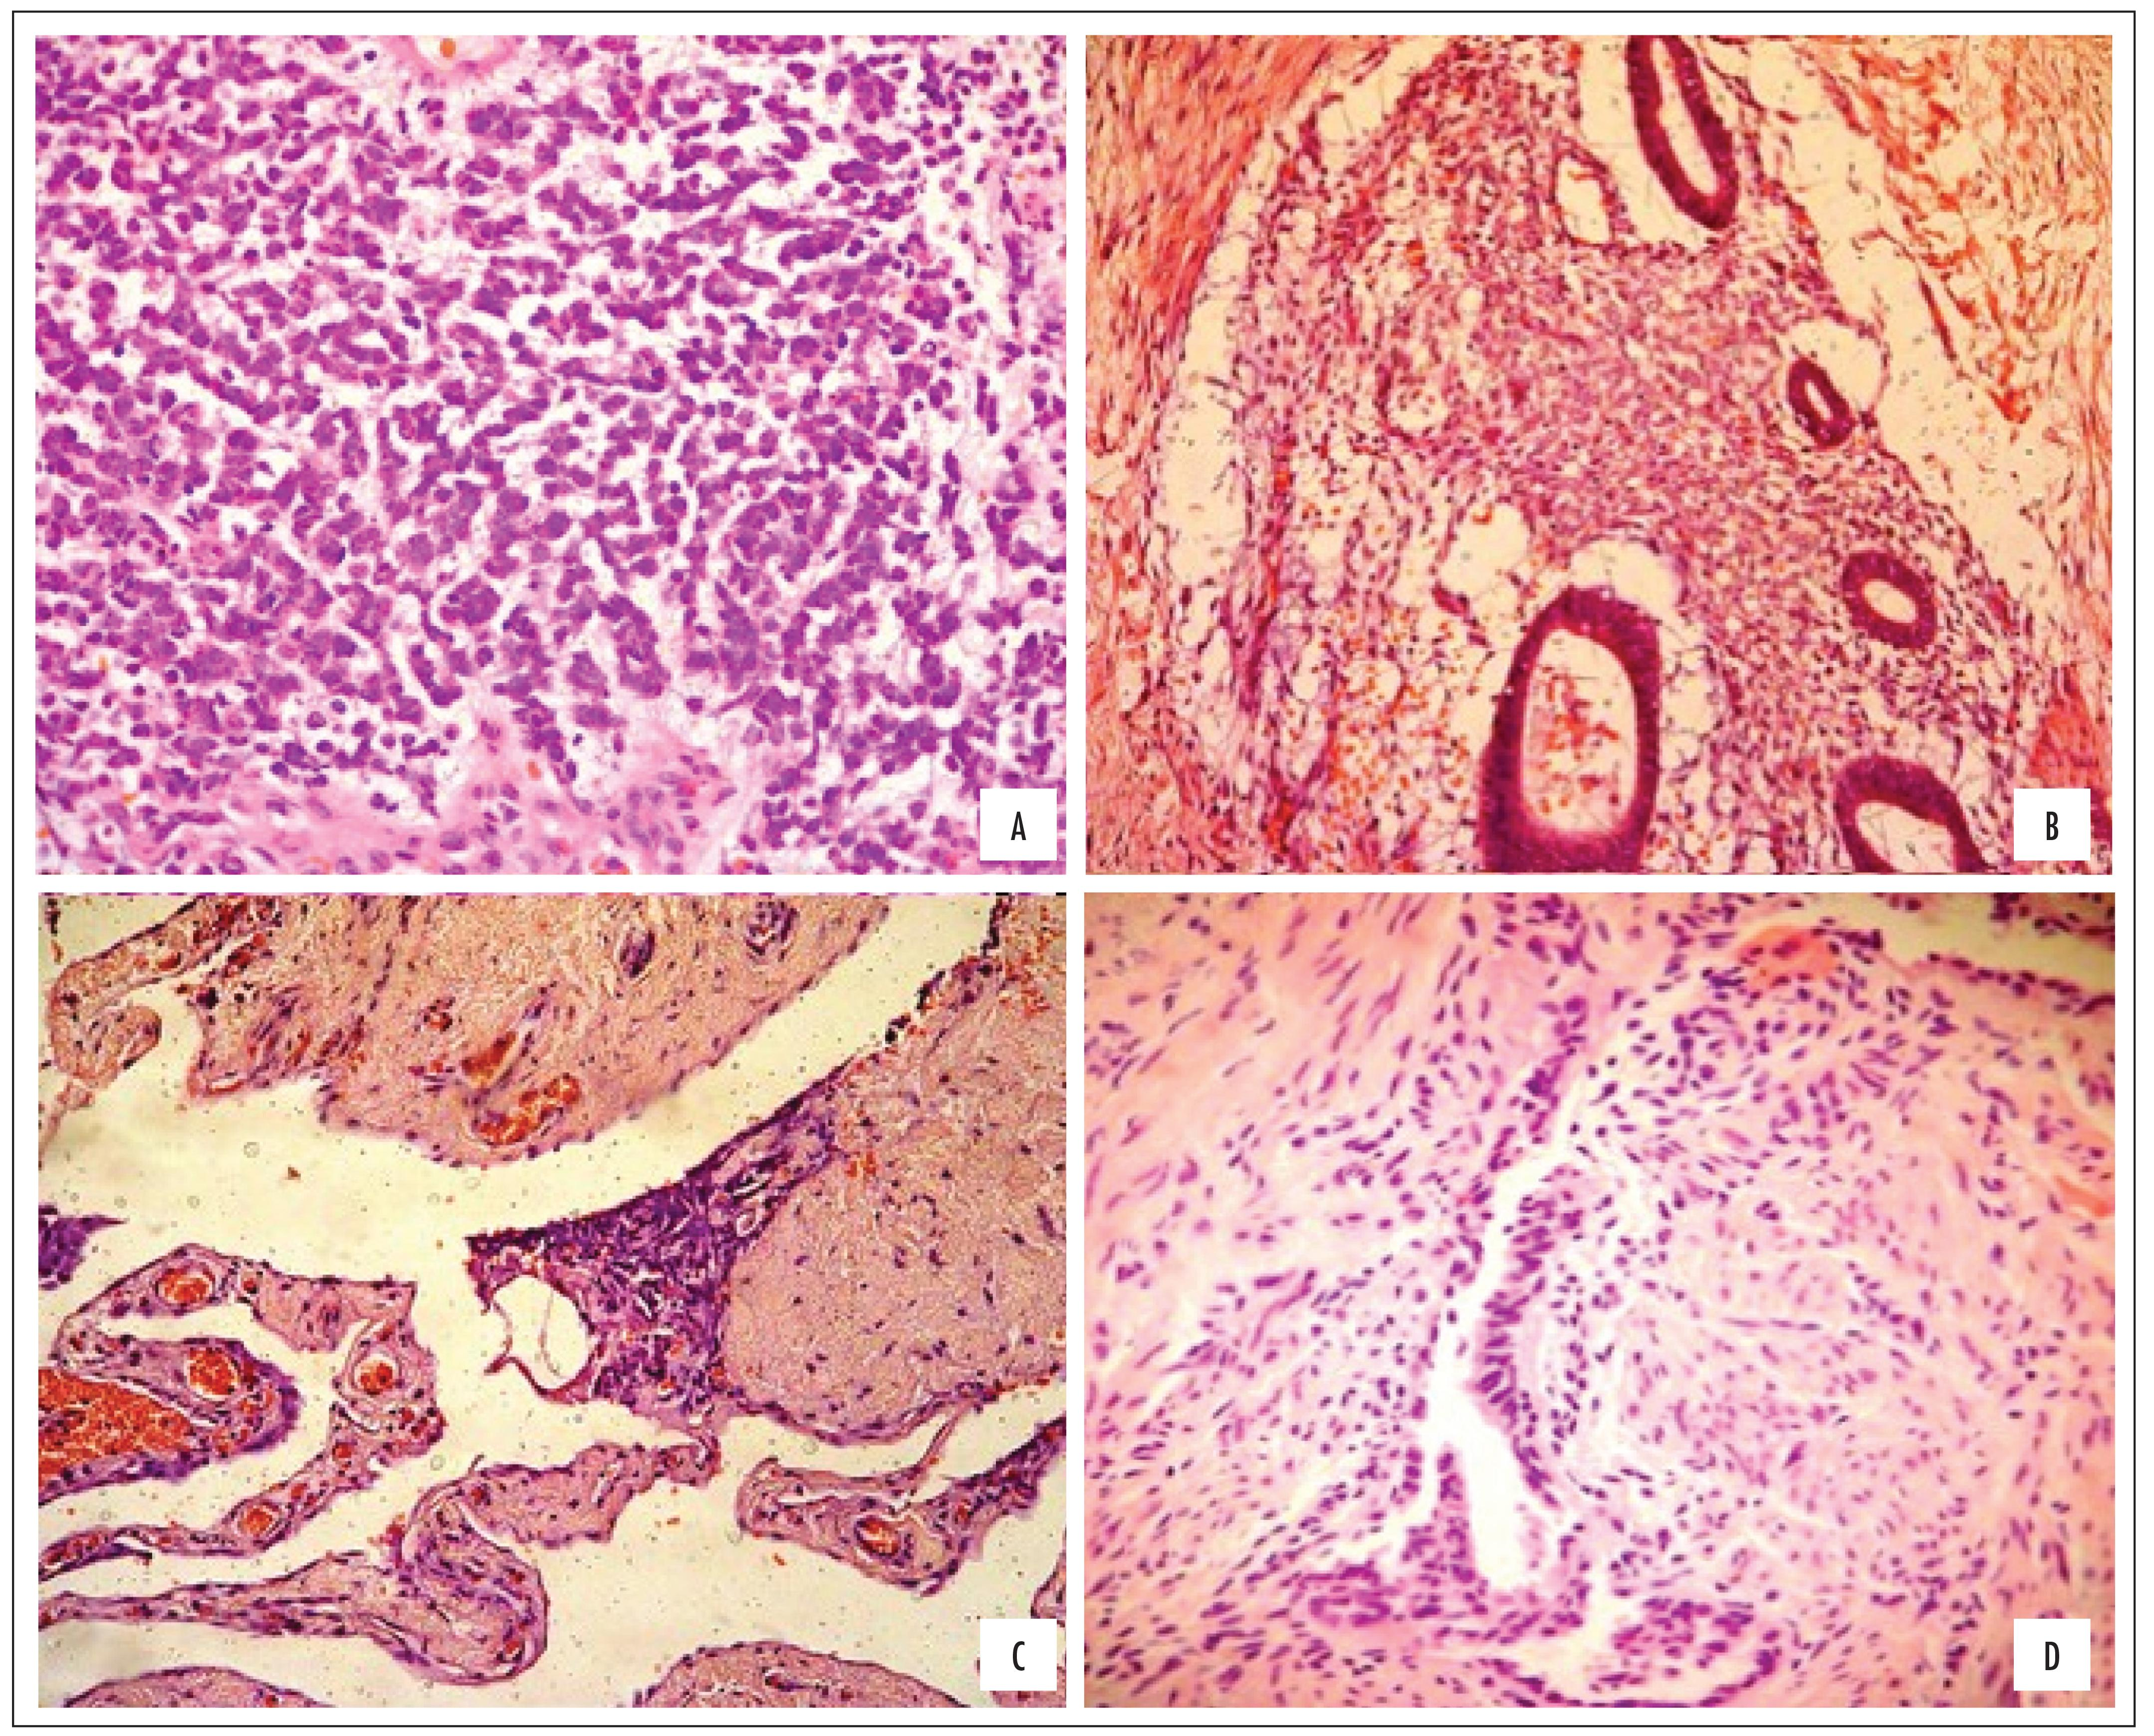
\includegraphics[width=10cm]{citoendometriose1636.jpg}
\caption[Amostras histológicas de diversos tipos de endometriose]{Lâminas mostrando padrão histológico dos diversos tipos de endometriose. (A) endometriose estromal ; (B) endometriose glandular bem diferenciada ; (C) endometriose glandular indiferenciada; (D) endometriose glandular mista.(Disponível em Porto e Cols, 2015)}
\label{histologico}
\end{figure} 


\subsubsection{Infiltração}

Os implantes endometriais, de acordo com seu crescimento e evolução,
podem apresentar-se de formas distintas, podendo ser classificadas
como: superficiais ou peritoneais, quando as lesões são muito pequenas
com o tamanho de até 2mm, geralmente não aparecem em exames de imagem;
intermediária, para as lesões que atingem de 2mm a 4mm; profundas, os
implantes endometriais que atingem uma área igual ou superior a 5mm.
Essas lesões são, geralmente, compostas por células musculares,
epitélio glandular ativo e estroma escasso. E, podem causar uma reação
inflamatória e até fibrose nos tecidos adjacentes (American Society
for Reproductive Medicine, 1997).

Koninckx e Martin, 1992 categorizou a endometriose da seguinte forma:

\begin{itemize}
\item Tipo I --- é caracterizada por uma lesão com maior diâmetro na
  superfície peritoneal, que habitualmente se apresenta com aspectos
  esbranquiçados.
\item Tipo II --- nas lesões peritoneais, o reto encontra-se aderido ao
  fundo de saco de Douglas e ligamentos uterossacros.
\item Tipo III --- o implante endometrial caracteriza-se como tendo
  seu maior diâmetro abaixo da superfície do peritôneo, de forma
  esférica, e sua localização fica no septo reto-vaginal, onde
  aparecem como nódulos palpáveis.
\end{itemize}

\subsubsection{Severidade e o comprometimento dos órgãos}

De acordo com Acosta e Cols, 1973, a endometriose pode ser:

\begin{itemize}
\item Endometriose leve: lesões não associados com cicatrizes e
  retração do peritôneo, no fundo de saco anterior ou posterior ou no
  peritôneo pélvico.
\item Endometriose moderada: afeta um ou ambos os ovários com diversas
  lesões superficiais, com formação de cicatrizes ou pequenos
  implantes endometriais. Com aderências periovarianas mínimas,
  associadas a lesões do ovário.
\item Endometriose acentuada: lesões que afetam um ou ambos os ovários
  com endometriomas superiores a 2cm e lesões afetando uma ou ambas as
  trompas, obstruídas por implantes endometriais com aderência ou
  lesão associada a endometriose.
\end{itemize}

\subsection{Teorias}

A fisiopatologia da endometriose permanece desconhecida, embora muitas
teorias foram desenvolvidas para tentar justificar a presença do
tecido endometrial fora do seu local de origem. Como:

\begin{itemize}
\item Teoria da menstruação retrógrada
\item Teoria da metaplasia celômica
\item Teoria da disfunção imunológica
\end{itemize}


\subsubsection{Teoria da menstruação retrógrada}

Até hoje a teoria da menstruação retrógrada é a teoria mais
aceita. Ela foi descrita por Sampson em 1920, e afirma que a
implantação do tecido do endométrio fora da cavidade uterina se dá
através da regurgitação do sangue menstrual pelas trompas de Falópio e
acabam chegando no peritônio. Onde essas células provocam reação
inflamatória e dor nos períodos menstruais. Inclusive, observou-se que
a incidência de endometriose é maior em mulheres que tem refluxo
tubário, porém, nem todas as mulheres que possuem menstruação
retrógrada sofrem de endometriose, levando a crer que a patogenicidade
da doença pode ser um mecanismo multifatorial (Macer e Taylor, 2013).

\subsubsection{Teoria da metaplasia celômica}

A teoria da metaplasia celômica foi proposta por Mayer em 1919 e
retificada por Nisolle e Cols, 1997. Mayer propôs essa teoria com base
no fato de que o peritôneo e endométrio eutópico tem a mesma origem
embrionária. Deste modo, estes tecidos, mediante a estímulos
hormonais, teriam a capacidade de se diferenciar em células estromais
e glandulares características do epitélio endometrial eutópico,
sugerindo assim a origem dos focos de endometriose.

\subsubsection{Teoria da disfunção imunológica}

Esta teoria ajuda a explicar por que algumas mulheres com menstruação
retrógrada desenvolvem endometriose enquanto outras não. Pesquisas
mostraram que mulheres com endometriose tem imunidade alterada,
suportando a teoria de que a patogênese da endometriose pode estar
envolvida com uma resposta imune deficiente (Sinaii e Cols, 2002).

Pacientes com endometriose tem uma concentração mais elevada de
macrófagos ativados, diminuição da imunidade celular e repressão das
células NK (Sikora e cols, 2011; Osuga e Cols, 2011).

As lesões endometrióticas desencadeiam uma resposta inflamatória,
recrutando macrófagos e leucócitos ativados no local (Kyama e Cols,
2009). Esta resposta inflamatória pode impedir a eliminação dos
resquícios menstruais provenientes da menstruação retrógrada e
consequentemente promover a implantação e o crescimento das células do
endométrio nos locais ectópicos (Christodoulakos e Cols, 2007).

De acordo com (Ulukus e Arici, 2005) tanto as células do sistema imune
quanto as células endometriais secretam citocinas e fatores de
crescimento os quais induzem a proliferação celular e a angiogênese,
promovendo assim a implantação e o crescimento das lesões
endometriais.

\subsection{Sintomas} 

Os aspectos clínicos da doença consistem em dismenorreia grave,
dispareunia e dor pélvica em decorrência de sangramentos e aderências
intrapélvicas. Dores durante a defecação indicam envolvimento da
parede retal e disúria no envolvimento da bexiga. E, quando a doença
afeta o intestino delgado pode também ocasionar perturbações
intestinais (Robins e Cotran , 2010).

A sintomatologia da endometriose é bastante variada e autores afirmam
que não há relação entre os aspectos das lesões e os sintomas da
doença (Martin e Cols , 1989).  De acordo com um estudo realizado por
Hedyeh Riazi e Cols, 2015, os sintomas associados a esta patologia são
diversos e variam de acordo com o diagnóstico clinico de cada
paciente. Os sintomas mais comuns relatados da endometriose são: Dores
que se agravaram ao longo do tempo, descritas como dores pélvicas
durante o ciclo menstrual, dores ao ter relações sexuais, dor lombar,
dor retal ao evacuar no período menstrual, infecções no trato
urinário, inchaço, enxaqueca, cansaço, febre, sangramentos,
infertilidade, distúrbios digestivos, náuseas, dores no estômago,
candidíase, doença inflamatória pélvica, cistos ovarianos, tonturas,
fadiga crônica.

Quando os implantes endometriais estão presentes na bexiga, os
sintomas característicos são hematúria e disúria. A hematúria cíclica
é uma característica importante da endometriose na bexiga, porém só
está presente em 20\% das pacientes (Akpınar e Cols, 2015).

Segundo Gao X e Cols, 2006, pacientes com endometriose podem
desenvolver transtornos psicológicos como ansiedade e depressão.
Deste modo, estes sintomas associados geram impacto negativo no bem
estar físico, mental e social da mulher, impedindo-a de realizar
atividades de sua vida cotidiana, diminuindo sua qualidade de vida e
desempenho sexual (Fourquet e Cols, 2011).

A endometriose também pode ser assintomática, como a endometriose
intestinal que aparece como implantes serosos e ocorre em 3\% a 37\% % 3% a 37% ? 30% a 37% ou 3% a 3,7%?
dos pacientes com endometriose (Pisanu e Cols, 2010).

Os pacientes com endometriose tendem a desenvolver sintomas
adicionais, tais como alergias, fibromialgia, asma, eczema, doença
inflamatória autoimune, síndrome da fadiga crônica e hipotireoidismo
(Sinaii e Cols, 2002).

Há também um maior risco de câncer de mama em mulheres diagnosticadas
com endometriose após os 40 anos, devido à sua maior exposição ao
estrogênio endógeno elevado (Bertelsen e Cols, 2007).

\subsection{Diagnóstico}

A endometriose é uma doença debilitante que pode causar vários
problemas na vida da mulher, entretanto, quando diagnosticada
precocemente, ela pode ser tratada e seus sintomas diminuídos.  Embora
o diagnóstico definitivo da endometriose necessite de uma intervenção
cirúrgica, preferencialmente por videolaparoscopia, diversos achados
nos exames físico, de imagem e laboratoriais já podem predizer, com
alto grau de confiabilidade, que a paciente apresenta endometriose.

\subsubsection{Diagnóstico Clínico}

A investigação inicial da endometriose é feita por meio de uma
anamnese para avaliação dos sintomas clínicos. Vale lembrar que o grau
de severidade da doença não está relacionado com os sintomas.
Entretanto, o diagnóstico da endometriose se torna difícil de se
confirmar devido a variabilidade de sintomas, bem como a correlação
não confiável entre a apresentação clínica e os achados cirúrgicos
(Wellbery, 1999), pois, esses sintomas podem estar relacionados com
outras condições patológicas como a síndrome do intestino irritável e
doença inflamatória pélvica. Por isso, muitas vezes, há um atraso de
vários anos entre o início dos sintomas e o diagnóstico definitivo
(Hadfield e Cols, 1995; Arruda e Cols 2003). Segundo Kundu e Cols,
2015 esse atraso no diagnóstico se dá também pela má relação entre
médico e paciente, pois de acordo com relatos das pacientes portadoras
da doença, muitos médicos não levam a sério as condições clínicas
delas, dificultando seu diagnóstico.

Há uma grande variedade de sintomas dolorosos que podem estar
relacionados à aparência, ao grau de invasão, à localização e à
profundidade de acometimento das lesões. São seis os sintomas que
devem ser investigados: dismenorréia, dispareunia, dor pélvica
acíclica, infertilidade e alterações urinárias e intestinais cíclicas.

Os sinais e sintomas associados ao exame clínico ginecológico já podem
dar uma ideia da presença da doença e do comprometimento dos órgãos
pélvicos, como é o caso da endometriose profunda infiltrativa, cujos
sinais sugestivos são nodulações palpáveis no fórnice vaginal
posterior ou septo retrovaginal, espessamento dos ligamentos
uterossacros ou lesões na vagina (Kennedy e Cols, 2005).

Esterilidade, irregularidade menstrual e dispaurenia (profunda) são
outras queixas. Em princípio, qualquer sinal ou sintoma que surja ou
se agrave no período menstrual tais como hematúria (menúria), disúria,
urgência miccional, polaciúria, dor ou sangramento à evacuação,
diarréia, deve nos sugerir diagnóstico de endometriose. O exame físico
pode ser aparentemente normal ou revelar nódulos na vagina, colo,
septo reto-vaginal e outros, espessamento (paramétrio), útero com
mobilidade reduzida, e doloroso à mobilização, massas anexiais.

Se o paciente estiver com sintomas de dor sugestivos de endometriose,
este deve ser tratado sem um diagnóstico definitivo, e exames
adicionais devem ser solicitados.
 
\subsubsection{Diagnóstico laboratorial}

Podemos utilizar também exame de sangue para pesquisa da presença do
CA-125. O CA-125 é um marcador da endometriose, ou seja, ele esta
presente na corrente sanguínea em níveis superiores aos normais,
quando a paciente está com doença em atividade, e se ele estiver com
nível superior a 100 U/ml, é indicativo de endometriose avançada,
muitas vezes já com comprometimento intestinal.

O CA-125, anticorpo monoclonal contra antígenos do epitélio ovariano,
não é específico, podendo surgir também em outros tumores de linhagem
epitelial, em, por exemplo, enfermidades hepáticas. Na endometriose
avançada pode se elevar a níveis superiores a 100U/ml. Ele deve ser
dosado no soro no período menstrual.

\subsubsection{Laparoscopia}

% padrão ouro?!
Considerado padrão ouro, a laparoscopia é uma técnica cirúrgica eficaz
com o objetivo de excisão endometriose visível e confirmação através
de exame histológico. Embora a comparação citológica seja padrão para
o diagnóstico da endometriose, algumas lesões visualizadas durante a
cirurgia não são examinadas em biópsia por que a visualização direta é
suficientemente característica (Adamson e Nelson, 1997). Como a
endometriose é uma condição crônica, é comum haver reincidência.

A laparoscopia é um procedimento cirúrgico onde o paciente é
anestesiado por uma anestesia geral --- uma pequena incisão é feita
perto do umbigo e um laparoscópio, tubo iluminado flexível, é inserido
nessa incisão. Com o laparoscópio é possível examinar e procurar
possíveis implantes endometriais nos órgãos abdominais do paciente com
possíveis implantes endometriais no abdome do paciente.

É importante notar que nem todas as lesões de endometriose são
visualizadas no momento da cirurgia; lesões podem estar escondidos por
órgãos ou aderências pélvicas, microscópico ou semelhantes na
aparência com outras lesões malignas ou benignas, como o câncer de
ovário, hemangioma ou gravidez ectópica (Brosens e Cols, 2004).

\subsubsection{Diagnóstico por métodos de imagem}

\paragraph{Ultrassonografia } 

% Não está mto bom no final do parágrafo
Por ser de custo acessível, ausência de radiação ionizante e fácil
acesso, a ultrassonografia transvaginal é o primeiro exame de imagem a
ser solicitado para a paciente com histórico e exame físico sugestivo
de endometriose (Fleischer e Cols, 1996). Preferencialmente com
preparo intestinal, que tem por objetivo eliminar os resíduos fecais e
gases eventualmente presentes no intestino, que possam atrapalhar a
identificação das lesões de endometriose encontradas no reto, sigmoide
regiões retrocervical e septo retovaginal. Um estudo de Abrão e
Cols, 2007, avaliando o exame, demonstrou uma sensibilidade de 94\% e
uma especificidade de 98\% na identificação de focos de endometriose
profunda.

Bazot e Cols, 2003, demonstrou que a ultrassonografia transvaginal foi
tão eficiente quanto a transretal endoscópica, tanto para o
diagnóstico quanto para a avaliação da extensão da endometriose retal.

% Esse também não está legal
Para avaliação de endometriose intermediária ou profunda, a
ultrassonografia transvaginal é um método eficiente (Moore e Cols,
2012). Como relatado por Fedele e Cols, 1997, essa técnica é
recomendada para o diagnóstico de endometriomas e endometriose da
bexiga, porém, quanto a avaliação de lesões superficiais peritoneais
ou focos de endometriose no ovário, o uso da ultrassonografia como
diagnóstico ainda é inconclusivo.

Segundo Bazot e Cols, 2003, a principal limitação das técnicas de
ultrassonografia é a falta de amplitude da área estudada, pois elas
se concentram em uma área anatômica limitada da cavidade pélvica.

\paragraph{Ressonância Nuclear Magnética (RNM)}

A ressonância nuclear magnética (RNM) é recomendada para complementar
o diagnóstico da endometriose pélvica. As principais indicações estão
relacionadas ao estadiamento da doença, ou seja, na maneira de avaliar
a extensão da endometriose em relação ao órgão no qual se originou, e
na análise de imagens duvidosas no estudo com o ultra-som.

A RNM foi recentemente usada para o diagnóstico em que os ligamentos
sacro uterinos revelaram falta de sensibilidade para o diagnóstico da
doença com envolvimento retal (Kinkel e Cols, 1999). % Envolvimento?

No estudo realizado por Bazot e Cols, 2003, com pacientes que foram
submetidos a RNM, eles obtiveram uma sensibilidade de 90,3\% e
especificidade de 91\%. Também fizeram uma comparação de RNM e
achados cirúrgicos patológicos de pacientes com endometriose pélvica
comprovada onde foram observadas áreas de tecidos correspondente a
fibrose, característico de endometriose. Quando a RNM foi comparada
com a ultrassonografia transvaginal, a RNM mostrou-se mais específica,
pois era capáz de fazer uma avaliação mais ampla da pélvis. Porém,
quando a endomeriose pélvica profunda está localizada no cólon
sigmóide, pode ser confundido com material fecal, sendo assim, o uso
de enema antes da RNM é útil para o diagnóstico neste local (Kinkel e
Cols, 1999).


\paragraph{Eco-colonoscopia}

Indicado especialmente em casos de suspeita de endometriose envolvendo
o intestino. Baseia-se na realização de um ultra-som por via
transretal, associado a um exame de colonoscopia. Desta forma, tem-se
uma imagem que pode indicar a presença da endometriose e, permite
ainda avaliar as camadas de intestino acometidas pela doença. No
entanto, é um exame mais invasivo quando comparado a outros exames como
o ultra-som com preparo intestinal e a ressonância, além de estar
limitado à avaliação apenas do intestino

\subsection{Perspectivas para um novo diagnóstico da endometriose}




\subsection{Tratamento} 

O tratamentos para a endometriose é individualizado e depende da
intensidade dos sintomas, assim como da evolução das lesões. Sendo
assim, o tratamento pode envolver tanto a intervenção farmacológica
como a cirúrgica, lembrando que dependendo do paciente e do estágio
das lesões esses procedimentos são feitos de forma integrada(Hernando
e Cols, 2015). Os tratamentos médicos farmacológicos disponíveis para
a endometriose incluem: contraceptivos orais, análogos de GnRH,
análogos de progesterona e inibidores da aromatase. Cada um desses
medicamentos tem suas especificidades e cabe ao médico avaliar a
gravidade da doença para prescrever a melhor forma de tratamento para
cada caso individualizado (Braundmeier e Fazleaba, 2009).

A forma de tratamento para a endometriose pode ser dividida em três
categorias: alívio da dor, supressão endometrial e cirurgia (Mattson e
Matfin ,2010). A escolha do tratamento dependerá da gravidade dos
sintomas, da extensão, localização da doença, do desejo de engravidar
e da idade da paciente.

Ainda há uma necessidade de novos medicamentos para tratamento da
endometriose que reduza a dor pélvica, minimize a intervenção
cirúrgica e preserve a fertilidade (Hernando e Cols,2015).

% recidivas está certo?
A endometriose pode retornar independente do tratamento, exceto da
cirurgia radical, e, esse retorno pode estar associada com a gravidade
da doença. Com tratamento clínico, as taxas de recidivas da doença
depois de 7 anos variam de 34\% em mulheres com doença leve e até 74\%
em mulheres com doença grave. Foram, também, relatadas taxa de
recidivas de 20 a 40\% dentro de 5 anos após cirurgia (Mattson e
Matfin ,2010) .

\subsubsection{Análogos de GnRH}

Sabe-se que o GnRH, hormônio liberador de gonadotrofinas, é um
hormônio liberado de forma pulsátil, em média de 5 a 25 minutos de
duração. É secretado pelo hipotálamo e age sobre a hipófise, levando
como resposta a liberação de LH e FSH, o hormônio luteinizante e
hormônio folículo estimulante, respectivamente.

Ele é responsável por regular indiretamente a atividade gonadal por
meio da liberação do LH e do FSH (Guyton e Hall, 2006). Deste modo, os
antagonistas de GnRH tem como principal mecanismo de ação inibir os
receptores competitivos de GnRH, já os agonistas de GnRH provocam uma
liberação inicial de gonadotrofinas, seguida de uma dessensibilização
gonadotrópica e desregulação da sinalização intracelular. Sendo assim,
Huirne e Lambalk, 2001, mostraram que a utilização de antagonistas de
GnRH devem possivelmente ser tão eficaz quanto a utilização de um
agonista de GnRH no tratamento da endometriose.  Alguns fármacos mais
utilizados como análogos de GnRH no tratamento da endometriose são a
Leuprolida e a Goserelina, conhecido como Roladex, eles são eficazes % é conhecido como roladex ou é outra coisa?
no melhoramento da dor das pacientes com endometriose, entretanto,
essas medicações tem provocado efeitos adversos, como suores noturnos
e a diminuição significativa de massa óssea (Schrager e Cols, 2013).

\subsubsection{Danazol}

Danazol é um fármaco utilizado no tratamento da endometriose por ter
se mostrado eficaz no combate a dores pélvicas associadas à
endometriose. Ele pode ser administrado tanto por via oral ou por via
vaginal, através de anéis vaginais, cremes ou dispositivos
intrauterinos, porém, sua utilização ainda é limitado por causar
efeitos colaterais androgênicos significativos como ganho de peso,
acne, seborreia e pelos excessivos pelo corpo --- hirutismo.

Estudos realizados por Cottreau e Cols 2003, mostraram uma associação
entre o uso do danazol e o aparecimento de câncer no ovário. Os
autores sugerem que os andrógenos circulantes com o uso do danazol
podem estar envolvidos no desenvolvimento do câncer ovariano, pois foi
observado uma grande expressão de receptores androgênicos na maioria
dos tumores nos ovários.

\subsubsection{Inibidores da aromatase ( IAs )}

Como a endometriose é considerada uma doença crônica dependente de
estrogênio, inibidores da aromatase são utilizados no tratamento da
doença como o Anastrozol e o Letrozol. Aromatazes são enzimas que
convertem andrógenos adrenais em estrogênio (Almassinokiani e Cols,
2014), e esses inibidores utilizados tem como mecanismo de ação inibir
esta enzima bloqueando a conversão e suprimir os níveis de estrogênio
em tecidos de endometriose. Os IAs são utilizados para tratar as dores
pélvicas provenientes da endometriose, reduzindo os tamanhos das
lesões. Ele também mostrou ser eficaz quando administrado em conjunto
com os análogos de GnRH em mulheres que mostraram resistência aos
tratamentos convencionais (Usluogullari e cols ,2015).


\subsubsection{Tratamento cirúrgico}

Quando o tratamento medicamentoso e hormonal não surtem os efeitos
desejados, a cirurgia pode ser necessária para aliviar a dor e
aumentar possibilidade de gestação.  O tratamento cirúrgico da
endometriose compreende desde procedimentos de baixa complexidade,
como a cauterização de focos superficiais e liberação de aderências, até
intervenções complexas nos ovários, fundo de saco de Douglas,
intestino, bexiga e ureteres (Guo, 2009). Além disso, muitas pacientes
apresentam infertilidade associada à dor, exigindo que o procedimento
cirúrgico seja conservador. Entretanto, é importante que tanto o
médico quanto a paciente estejam cientes de que a cirurgia
conservadora implica índices elevados de recorrência da doença. % recorrência da dor ou da doença? estava dor, troquei

Para a paciente com infertilidade associada a endometriose de grau
mínimo e leve, a ablação dos focos e a adesiólise mostrou-se eficaz,
melhorando a fertilidade (Jacobson e Cols, 2002).

% Não está mto bom
Para os pacientes com endometriomas ovarianos e que não respondem
adequadamente ao tratamento medicamentoso, a cirurgia é indicada nos
casos de endometriomas sintomáticos ou grandes (Chapron e Cols, 2002).

\subsection{Reincidência}

% Ta estranho esse paragrafo
Morgante e Cols, 1999, relataram que os pacientes tratados com baixa
dose de danazol, por exemplo, 100 mg por dia, durante 6 meses, após a
cirurgia laparoscópica, e então seis meses de terapia com GnRH
agonistas, reduziram a incidência de dor pélvica quando comparados com
aqueles que não receberam a terapia. Especificamente, 24 meses após a
cirurgia, os 14 pacientes escolhidos aleatoriamente para receber o
tratamento com danazol tiveram a dor reincidida, porém foi
significativamente menor do que os outros 14 pacientes que não
receberam qualquer tratamento.

\section{Referências} 

COX, H, HENDERSON, L., ANDERSEN,N., CAGLIARINI , G, e SKI.C(2003). Fucus group of endometriosis: Struggle, loss and the medical merry-go-round. Internetional journal of nurseng practice , 9,2-9

GUYTON; Fisiologia Humana; Sexta edição; Rio de Janeiro; Editora Guanabara
Koogan, 2011; 545 p.

GUYTON e HALL; Tratado de Fisiologia Médica; Décima primeira edição; Rio de
Janeiro; Editora Elsevier, 2006; 1011 p.

SILVERTHORN; Fisiologia humana ; Quinta edição; São Paulo; Editora Artmed, 2010; 848 p.

Viganò P, Somigliana E, Panina P, Rabellotti E, Vercellini P, Candiani M.Principles of phenomics in endometriosis.Hum Reprod Update. 2012 May-Jun;18(3):248-59

Verkauf BS. Incidence, symptoms, and signs of endometriosis in fertile and infertile women. J Fla Med Assoc. 1987

Kelechi E. Nnoaham, Sivahami Sivananthan, Lone Hummelshoj, Crispin Jenkinson, Premila Webster, Stephen H. Kennedy, and Krina T. Zondervan. MULTI-CENTRE STUDIES OF THE GLOBAL IMPACT OF ENDOMETRIOSIS AND THE PREDICTIVE VALUE OF ASSOCIATED SYMPTOMS.J Endometr. 2009; 1(1): 36–45. 

Kennedy S1, Bergqvist A, Chapron C, D'Hooghe T, Dunselman G, Greb R, Hummelshoj L, Prentice A, Saridogan E; ESHRE guideline for the diagnosis and treatment of endometriosis.Hum Reprod. 2005 Oct;20(10):2698-704. 


PORTH, M. C. e MATFIN, G.; Fisiopatologia; Oitava edição, volume 2; Rio de
Janeiro; Editora Guanabara Koogan, 2010; 1146 p.

GERALDO BRASILEIRO FILHO; Bogliolo Patologia; oitava edição; Rio de Janeiro; Editora Guanabara Koogan, 2011; 604 P.

THOMAS C. KING; Patologia; Primeira edição ; Rio de janeiro; Editora Elsevier, 2007; 347 P

KARP, JASON R., Marathon e Beyond , 2015, Vol. 19 Issue 2, p112 e 113.

ADRIANA ZANONA DA MATA E MARISA CAMPIO MULLER; Uma análise qualitativa da convivência da mulher com sua endometriose. Psicologia, saúde e doenças. 2006, 7 (1), 57-72

LAURA KNABBEN,SARA IMBODEN, BERNHARD FELLMANN,KONSTANINOS NIRGIANAKIS,ANNETTE KUHN, MICHAEL D. MUELLER. Urinary tract endometriosis in patients with deep infiltrating endometriosis: prevalence, symptoms, management, and proposal for a new clinical classification, 2014.

LENE N. HEIDEMANN , DORTHE HARTWELL , CHRISTIAN H. HEIDEMANN e KIRSTEN M.
JOCHUMSEN ; The relation between endometriosis and ovarian cancer – a
review;Acta Obstetricia Et Gynecologica Scandinavica ;2013

Sun Mi Hwang, Chung Won Lee, Byung Seok Lee, and Joo Hyun Park ; Clinical features of thoracic endometriosis: A single center analysis, 2015.

ZHAO DONGXU, YIN FEI, XIAO XING, ZHANG BO-YIN, ZHU QIN GSAN; Low back pain tied to spinal endometriosis, 2014


Hedyeh Riazi, Najmeh Tehranian,corresponding author Saeideh Ziaei,corresponding author Easa Mohammadi, Ebrahim Hajizadeh, and Ali Montazeri; Clinical diagnosis of pelvic endometriosis: a scoping review; 2015; 15-39

Audebert A, Bäckström T, Barlow DH, Benagiano G, Brosens I, Bühler K, Donnez J, Evers JL, Pellicer A, Mettler L, et al.Endometriosis 1991: a discussion document.Hum Reprod. 1992 Mar;7(3):432-5.

Kitawaki J, Kado N, Ishihara H, Koshiba H, Kitaoka Y, Honjo H.Endometriosis: the pathophysiology as an estrogen-dependent disease. J Steroid Biochem Mol Biol. 2002 Dec;83(1-5):149-55.

Noble LS, Simpson ER, Johns A, Bulun SE.Aromatase expression in endometriosis.J Clin Endocrinol Metab. 1996 Jan;81(1):174-9

Brosens I, Diagnosis of endometriosis.Semin Reprod Endocrinol. 1997;15(3):229-33

rosens I, Puttemans P, Campo R, Gordts S. Diagnosis of endometriosis: Pelvic endoscopy and imaging techniques. Best Practice and Research Clinical Obstetrics and Gynaecology. 2004;18(2):285–303.

American Society for Reproductive Medicine;Revised American Society for Reproductive Medicine classification of endometriosis: 1996

Beatriz Taliberti da Costa Porto , Helizabet Salomão Abdalla Ayrosa Ribeiro , Maria Antonieta Longo Galvão , Vanessa Gozzo Sekula , José Mendes Aldrigui , Paulo Augusto Ayrosa Ribeiro.
Histological classification and quality of life in women with endometriosis .2015

Martin DC, Hubert GD, Vander Zwaag R, el-Zeky FA. Laparoscopic appearances of peritoneal endometriosis.Fertil Steril 1989; 51:63-7

Francesco Antonio Viscomi, Rogério Dias, Laurival de Luca, Mauro Fernando Kürten Ihlenfeld. Correlation Between Laparoscopic Aspects and Histologic Findings in Peritoneal Endometriotic Lesions. Rev. Bras. Ginecol. Obstet. v.24 2002 .

Ulukus M, Arici A.Immunology of endometriosis.Minerva Ginecol. 2005 Jun;57(3):237-48.

Sinaii N, Cleary SD, Ballweg ML, Nieman LK, Stratton P.High rates of autoimmune and endocrine disorders, fibromyalgia, chronic fatigue syndrome and atopic diseases among women with endometriosis: a survey analysis.Hum Reprod. 2002 Oct;17(10):2715-24.

Christodoulakos G, Augoulea A, Lambrinoudaki I, Sioulas V, Creatsas G. Pathogenesis of endometriosis: the role of defective 'immunosurveillance'.Eur J Contracept Reprod Health Care. 2007 Sep;12(3):194-202.

Nisolle M, Donnez J. "Peritoneal endometriosis, ovarian endometriosis, and
adenomyotic nodules of the rectovaginal septum are three different entities."
Fertil Steril. 1997;68(4):585-96.

Redwine DB1.Age-related evolution in color appearance of endometriosis.Fertil Steril. 1987 Dec;48(6):1062-3.

Koninckx PR, Martin DC,Deep endometriosis: a consequence of infiltration or retraction or possibly adenomyosis externa?Fertil Steril. 1992 Nov;58(5):924-8.

Acosta AA, Buttram VC, Jr., Besch P K, Malinak LR, Franklin RR,
Vanderheyden JD. "A proposed classification of pelvic endometriosis."
Obstet Gynecol. 1973;42(1):19-25.


Arruda MS1, Petta CA, Abrão MS, Benetti-Pinto CL.Time elapsed from onset of symptoms to diagnosis of endometriosis in a cohort study of Brazilian women. Hum Reprod. 2003 Apr;18(4):756-9.

Hornstein MD1, Yuzpe AA, Burry KA, Heinrichs LR, Buttram VL Jr, Orwoll ES. Prospective randomized double-blind trial of 3 versus 6 months of nafarelin therapy for endometriosis associated pelvic pain.Fertil Steril. 1995 May;63(5):955-62.

Stephen Kennedy , Agneta Bergqvist  , Charles Chapron  , Thomas D’Hooghe  , Gerard Dunselman  , Robert Greb  , Lone Hummelshoj  , Andrew Prentice  , Ertan Saridogan .ESHRE guideline for the diagnosis and treatment of endometriosis. 2005.

Bazot M1, Detchev R, Cortez A, Amouyal P, Uzan S, Daraï E.Transvaginal sonography and rectal endoscopic sonography for the assessment of pelvic endometriosis: a preliminary comparison.Hum Reprod. 2003 Aug;18(8):1686-92. (A)

Marc Bazot, Emile Darai, Roula Hourani, Isabelle Thomassin, Annie Cortez, Serge Uzan, 
Jean-Noe l Buy, MDDeep Pelvic Endometriosis: MR Imaging for Diagnosis and Prediction of Extension of Disease 1 (B).


Moore J, Copley S, Morris J, Lindsell D, Golding S, Kennedy S. A .systematic review of the accuracy of ultrasound in the diagnosis of endometriosis. Ultrasound Obstet Gynecol. 2002 .

Fedele L1, Bianchi S, Raffaelli R, Portuese A. Pre-operative assessment of bladder endometriosis. Hum Reprod 1997; 12:2519 –2522.

Kinkel K1, Chapron C, Balleyguier C, Fritel X, Dubuisson JB, Moreau JF.. Magnetic resonance imaging characteristics of deep endometriosis. Hum Reprod 1999; 14:1080 –1086.

Fleischer AC, Cullinan JW, Walsch JW. Problem-oriented gynecologic imaging with emphasis on usltrasonography. In Fleischer AC, Manning FA, Jeanty P, Romero R.(Ed.). Sonography in Obstetrics and Gynecology. A.
Lange. 1996;887.

Abrão MS, Gonçalves MO, Dias JA Jr, Podgaec S, Chamie LP, Blasbalg R. Comparison between clinical examination, transvaginal sonography and magnetic resonance imaging for the diagnosis of
deep endometriosis. Hum Reprod. 2007;22(12):3092-7


Jacobson TZ, Barlow DH, Koninckx PR, Olive D, Farquhar C. Laparoscopic surgery for subfertility associated with endometriosis. Cochrane Database Syst Rev. 2002;(4):CD001398.


Chapron C, Vercellini P, Barakat H, Vieira M, Dubuisson JB. Management of ovarian endometriomas. Hum Reprod Update. 2002;8(6):591-7.

Adamson GD, Nelson HP. Surgical treatment of endometriosis. Obstet Gynecol Clin North Am 1997; 24:375– 409.



Júlia Kefalás Troncon, Ana Carolina Tagliatti Zani, Andrea Duarte Damasceno Vieira, Omero Benedicto Poli-Neto, Antônio Alberto Nogueira, and Júlio César Rosa-e-Silva .Endometriosis in a Patient with Mayer-Rokitansky-Küster-Hauser Syndrome . Case Rep Obstet Gynecol. 2014

Matthew Latham Macer, M.D. and Hugh S. Taylor. Endometriosis and Infertility: A review of the pathogenesis and treatment of endometriosis-associated infertility 2013.

A.G. Braundmeier and A.T. Fazleabas. The non-human primate model of endometriosis: research and implications for fecundity. 2009.

Jessica Fourquet, Xin Gao, Diego Zavala, Juan C. Orengo, Sonia Abac, Abigail Ruiz, Joaquín Laboy, and Idhaliz Flores Patients’ report on how endometriosis affects health, work, and daily life, 2011.


ADOLFO PISANU, DANIELA DEPLANO, STEFANO ANGIONI, ROSSANO AMBU E ALESSANDRO UCCHEDDU. Rectal perforation from endometriosis in pregnancy: Case report and literature review, World J. Gastroenterol. 2010 .

Gao X, Yeh YC, Outley J, Simon J, Botteman M, Spalding J. Health-related quality of life burden of women with endometriosis: a literature review. Curr Med Res Opin. 2006.

S. Kundu, J. Wildgrube, C. Schippert, P. Hillemanns, and I. Brandes.Supporting and Inhibiting Factors When Coping with Endometriosis From the Patients Perspective. Geburtshilfe Frauenheilkd. 2015.

Süha Akpınar, Güliz Yılmaz,corresponding author and Emre Çelebioglu. A rare cyclic recurrent hematuria case; bladder endometriosis.Quant Imaging Med Surg. 2015 

Huirne JA, Lambalk CB.Gonadotropin-releasing-hormone-receptor antagonists.Lancet. 2001.

Wellbery C. Diagnosis and treatment of endometriosis. American Family Physician. 1999;60(6):1753–1762.

Leticia Muñoz-Hernando, Jose L Muñoz-Gonzalez, Laura Marqueta-Marques, Carmen Alvarez-Conejo, Álvaro Tejerizo-García, Gregorio Lopez-Gonzalez, Emilia Villegas-Muñoz, Angel Martin-Jimenez, and Jesús S Jiménez-López. Endometriosis: alternative methods of medical treatment.Int J Womens Health. 2015; 7: 595–603. 

Schrager S, Falleroni J, Edgoose J. Evaluation and treatment of endometriosis.Am Fam Physician. 2013

Gabriella Zito, Stefania Luppi, Elena Giolo, Monica Martinelli, Irene Venturin, Giovanni Di Lorenzo, and Giuseppe Ricci .Medical Treatments for Endometriosis-Associated Pelvic Pain.Biomed Res Int. 2014.

Cottreau CM, Ness RB, Modugno F, Allen GO, Goodman MT. Endometriosis and its treatment with danazol or lupron in relation to ovarian cancer. Clin Cancer Res. 2003.

Fariba Almassinokiani, Alireza Almasi, Peyman Akbari, and Mahboubeh Saberifard.Effect of Letrozole on endometriosis-related pelvic pain.Med J Islam Repub Iran. 2014; 28: 107. 

Betul Usluogullari,corresponding author Candan Zehra Duvan, and Celil Alper Usluogullari.Use of aromatase inhibitors in practice of gynecology.J Ovarian Res. 2015.

Guo SW.Recurrence of endometriosis and its control.Hum Reprod Update. 2009 Jul-Aug;15(4):441-61.




\end{document}

%%% Local Variables:
%%% mode: latex
%%% TeX-master: t
%%% End:
